\section{Primordial spectra}\label{rep:spectra}

The turning point leaves no feature in the primordial spectra.
Every mode of the torus is deep inside the Hubble radius at the turn and starts in its adiabatic vacuum, which evolves into the Bunch--Davies state of the plateau.
The scalar tilt and the tensor-to-scalar ratio $\rT$ are therefore those of the plateau potential, Eq.~\eqref{eq:rA-plateau}, at the number of $e$-folds fixed by reheating.
Through the scale of inflation the spectra also enter the two observable consequences of the turn, the shape fossil and the Higgs criterion, but only weakly.
Section~\ref{rA:c-nofeature} treats tensors and scalars through the turn, Sec.~\ref{rA:c-tilt} the tilt and the tensor ratio, and Sec.~\ref{rA:c-scale} what the tensor ratio fixes.

\begin{figure}[tbp]
\centering
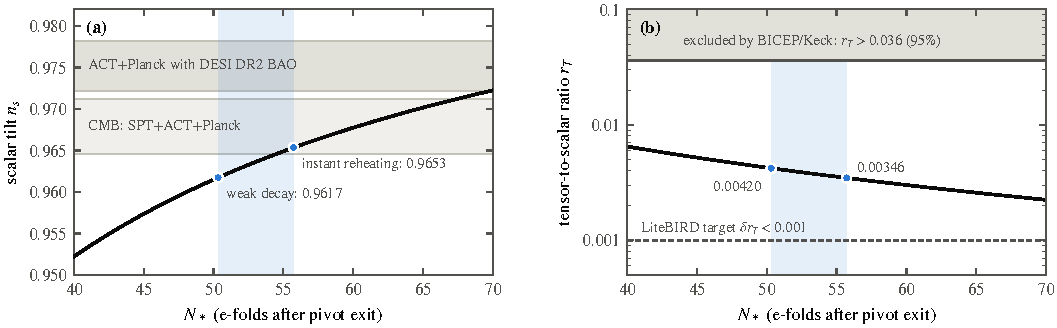
\includegraphics[width=\textwidth]{prd_primordial}
\caption{Primordial tilt and tensor ratio of the plateau potential, which the turning point leaves intact. (a)~Scalar tilt versus the number $N_*$ of $e$-folds between pivot exit and the end of inflation; the colored band spans the weak visible decay ($N_*=50.33$) and instant reheating ($55.72$). Gray bands: $68\%$ intervals from SPT-3G, ACT and Planck CMB data (CMB-SPA)~\cite{SPT-3G:2025bzu} and from ACT and Planck with CMB lensing and DESI DR2 baryon acoustic oscillations (P-ACT-LB2)~\cite{AtacamaCosmologyTelescope:2025blo,DESI:2025zgx}. (b)~Tensor-to-scalar ratio $\rT$ with the BICEP/Keck bound~\cite{BICEP:2021xfz} and the LiteBIRD target~\cite{LiteBIRD:2022cnt}.} %
\label{fig:rA-primordial}
\end{figure}

\subsection{No feature from the turning point}
\label{rA:c-nofeature}

All modes of the torus are inside the Hubble radius at the turn by at least a factor $k/(a_bh)=2\pi|\bm n|/(h\Lb)\geq2\pi/(h\Lb)\simeq1400$ (1300 for free fields), and the emptiness gate of Sec.~\ref{rep:gate} puts them in their adiabatic vacuum there. %
That vacuum evolves into the Bunch--Davies state of the subsequent plateau, with Bogoliubov coefficients suppressed by powers of $h\Lb/2\pi|\bm n|$.

\paragraph{Tensors.}
Free tensor modes $h_{\bm k}=v/a$ on the turning-point solution, Eq.~\eqref{eq:rA-turning-solution}, obey $v''+(k^2-a''/a)v=0$ with $a''/a=2h^2a^2$ exactly (Eq.~\eqref{eq:rA-app}).
With the lemniscatic form of the scale factor, Eq.~\eqref{eq:rA-lemniscatic}, $a^2=\Lb^2\wp(z)$ with $z=h\Lb(\eta-\eta_0)$ and invariants $g_2=4$, $g_3=0$, this is Lam\'e's equation with $n(n+1)=2$,
\begin{equation}
\frac{d^2v}{dz^2}=\Big[2\wp(z)-\frac{k^2}{(h\Lb)^2}\Big]v ,
\label{eq:rA-lame}
\end{equation}
the flat counterpart of the closed universe with radiation and a positive cosmological constant treated in Ref.~\cite{Sarangi:2006yy}.
For $n=1$ the solutions are known in closed form: Hermite's functions $v=\sigma(z+\alpha)\,e^{-z\zeta(\alpha)}/\sigma(z)$, with the Weierstrass functions $\sigma$ and $\zeta$, solve $v''=[2\wp(z)+\wp(\alpha)]v$, as follows from $(\ln v)''+[(\ln v)']^2$ and the addition theorem $[\zeta(z+\alpha)-\zeta(z)-\zeta(\alpha)]^2=\wp(z+\alpha)+\wp(z)+\wp(\alpha)$; here $\wp(\alpha)=-k^2/(h\Lb)^2$.
They are the Floquet (Bloch) solutions of Eq.~\eqref{eq:rA-lame}.
The far past and the far future are the two poles of $\wp$ that bound the real period, where $v\propto z^{-1}$ or $z^2$, the frozen and the decaying tensor mode of de~Sitter space.
For a ground state set at the turn, the late tensor power differs from that of the Bloch state of Lam\'e's equation, defined by its Floquet solutions, by $1.7\times10^{-6}$ at $k/(a_bh)=727$, below the lowest torus mode, and by $2\times10^{-7}$ at $2300$. %

\paragraph{Scalars.}
For scalars the variable $z_{\rm MS}=a\dot\phi/H$ of the Mukhanov--Sasaki equation is $0/0$ at $H=\dot\phi=0$, and its finite limit does not describe the inflaton at the turn.
A finite limit does not license the single-field equation.
For $V=V_b+\lambda(\phi-\phi_b)$ and $\lambda\to0$ the formal pump tends to $z_{\rm MS}''/z_{\rm MS}\to2a_b^2h_b^2/3$, while the decoupled field has $a''/a=2a_b^2h_b^2$, with $h_b^2=V_b/3\MPbar^2$. %
At a bounce some gauges become ill-defined while others stay regular~\cite{Allen:2004vz}; here the Newton-gauge variables continue regularly through the turning point.
We therefore use the regular Newton-gauge system for the inflaton perturbation $\delta\phi$ and the metric potentials $A$ and $\psi$, with the Casimir sector in its mean-contact truncation.
Its Ward identity requires the contact term $-2\rho_0U$, where $\rho_0$ is the comoving Casimir density and $U=A+\psi$.

On a reference plateau history with $\phi_b=5.587\,\MPbar$, states prepared about one $e$-fold before the turning point, at $a/a_b=2.67$, give late curvature power $1.0232$, $1.0236$ and $1.0241$ times the leading slow-roll prefactor at $k/(a_bh)=727$, $2300$ and $7270$. %
These ratios equal the first-order slow-roll values, $1.0226$--$1.0235$, plus higher orders. %
States prepared about one $e$-fold before the turn therefore reproduce the slow-roll normalization.
Second-order adiabatic states prepared five $e$-folds after the turning point, when the Casimir energy has diluted, reproduce them to $8\times10^{-4}$, $5\times10^{-7}$ and a few times $10^{-9}$. %
States prepared before the turn and after the dilution thus differ by $8\times10^{-4}$ at $k/(a_bh)=727$ and by a few times $10^{-9}$ at $7270$. %
Local preparations of lower adiabatic order differ by up to $4\times10^{-3}$ at $k/(a_bh)=727$. %
The finite Maxwell noise of the lowest gapped pair band contributes $1.5\times10^{-16}$. %
The gravitational coupling to the Casimir sector enters as $|\rho_C|/\MPbar^2k_{\rm phys}^2\lesssim4\times10^{-6}$. %
The scalar and tensor spectra on the torus are therefore those of plateau inflation, sampled on the reciprocal lattice.
During the plateau stage the Higgs field must also stay in its vacuum at all wavelengths; Sec.~\ref{rep:h-universality} compares that condition with the zero-mode condition at the turn.

\subsection{Tilt, tensors and reheating}
\label{rA:c-tilt}

The tilt and the tensor ratio then depend only on $N_*$, the number of $e$-folds between the exit of the pivot scale and the end of inflation.
We solve the exact mode equations of the plateau with second-order adiabatic initial states [Fig.~\ref{fig:rA-primordial}] and find $n_s=0.96534$ and $\rT=0.00346$ for instant reheating, $N_*=55.72$. %
For the weak visible decay through the reheating coupling of Sec.~\ref{rA:g-reheating}, $N_*=50.33$, they are $n_s=0.96174$ and $\rT=0.00420$. %
The tilts come from an independent exact mode solver, with second-order adiabatic initial states set $6$--$10$ $e$-folds before horizon exit. %
They are stable to $4\times10^{-8}$, and a zeroth-order initial state would bias $n_s$ by $-6\times10^{-4}$. %

\paragraph{Slow-roll cross-check.}
For the plateau of Eq.~\eqref{eq:rA-plateau}, with $e\equiv e^{-\sqrt{2/3}\,\phi/\MPbar}$, the slow-roll parameters are
\begin{equation}
\epsilon_V=\frac43\frac{e^2}{(1-e)^2},\qquad \eta_V=\frac43\frac{2e^2-e}{(1-e)^2},
\end{equation}
and to first order $n_s=1-6\epsilon_V+2\eta_V$ and $\rT=16\epsilon_V$ at the field value that lies $N_*$ e-folds, $N=\int d\phi/(\MPbar\sqrt{2\epsilon_V})$, before $\epsilon_V=1$.
This gives $n_s=0.96542$ and $\rT=0.00341$ at $N_*=55.722$, and $0.96181$ and $0.00414$ at $50.33$, within $10^{-4}$ in $n_s$ and $2\%$ in $\rT$ of the exact mode solution. %
The familiar leading estimates $1-2/N_*$ and $12/N_*^2$ are cruder, $0.9641$ and $0.0039$ at $N_*=55.72$. %

\paragraph{Reheating and the Casimir remnant.}
With the Standard Model as the only light content there is no hidden radiation to dilute, so reheating can proceed through ordinary couplings.
The Casimir sector is a negative radiation-like term with $|\rho_C|/\rho_\gamma\simeq6\times10^{-119}$ today for $L_0\simeq\dLSS$ with the high-energy weight, and about $13$ times less with only the photon and the graviton massless today, since their Casimir coefficient is $2\rAgam=3.35$ instead of $C=42.74$; its contribution to $\Delta N_{\rm eff}$ is negligible. %

\paragraph{Comparison with data.}
For instant reheating the tilt lies $0.8\sigma$ below the CMB-only value $n_s=0.9679\pm0.0033$ of SPT-3G, ACT and Planck combined (CMB-SPA, Table~I of Ref.~\cite{SPT-3G:2025bzu}), and for the weak decay $1.9\sigma$ below it. %
Adding DESI DR2 baryon acoustic oscillations to the same combination gives $n_s=0.9726\pm0.0028$ (Table~VI of Ref.~\cite{SPT-3G:2025bzu}; BAO data from Ref.~\cite{DESI:2025zgx}), and the offsets grow to $2.6\sigma$ and $3.9\sigma$; ACT and Planck with CMB lensing and DESI DR2 (P-ACT-LB2) give $0.9752\pm0.0030$~\cite{AtacamaCosmologyTelescope:2025blo}, $3.3\sigma$ and $4.5\sigma$ away. %
These are one-dimensional comparisons with published marginals; we evaluate no likelihood of the model.
The tension belongs to the plateau potential.
A potential with a larger tilt at the same $N_*$ changes these numbers and leaves the turning point intact, since the turn needs only $V(\phi_b)>0$ and the criterion~\eqref{eq:rA-exact-criterion}; its scale of inflation enters as described below.
The tensor ratio is an order of magnitude below the BICEP/Keck bound $\rT<0.036$~\cite{BICEP:2021xfz} and three to four times the LiteBIRD target $\delta\rT=10^{-3}$~\cite{LiteBIRD:2022cnt}. %

\subsection{What the tensor ratio fixes}
\label{rA:c-scale}

The scale of inflation enters both tests of the turning point, and only weakly.
The tensor power of two polarizations is $P_t=2H_*^2/(\pi^2\MPbar^2)$, so with $P_t=\rT A_s$
\begin{equation}
\frac{H_*}{\MPbar}=\pi\Big(\frac{A_s\rT}{2}\Big)^{1/2}.
\end{equation}
On the plateau the Hubble rate at pivot exit is $H_*\simeq0.986\,h$, so at fixed $A_s$ the scale $h$ grows as $\rT^{1/2}$ and, by Eq.~\eqref{eq:rA-scaling}, the width of the shape fossil as $\rT^{1/8}$. %
Measuring $\rT\simeq0.004$ to $\pm10^{-3}$ fixes $\sigma_E$ to $3.1\%$, and a precision of $5\times10^{-4}$ fixes it to $1.6\%$. %
Both are below the $5\%$ change of $\sigma_E$ per $0.02$ in $\fzm$ and the $10\%$ next-order shift (Sec.~\ref{rA:s-fossil}). %
At fixed $A_s$, lowering $\rT$ from about $0.004$ to $10^{-4}$ would lower $\sigma_E$ by the factor $(0.025)^{1/8}=0.63$. %
The Higgs criterion depends on the scale of inflation through the matching scale, $\mub=1/\Lb\propto h^{1/2}\propto\rT^{1/4}$ since $\Lb\propto h^{-1/2}$, and through the duration of the turn, which is set by $h\Lb\propto\rT^{1/4}$. %
Over the plateau class, $10^{-3}\leq\rT\leq10^{-2}$ at fixed $A_s$, the critical top mass at $\Pone=1/2$ moves by $\pm0.067\GeV$ (Sec.~\ref{rep:h-budget}). %
A measurement of $\rT$ therefore moves the predicted fossil by a few percent and the critical mass by a few hundredths of a GeV, and neither test hinges on it.
